%  article.tex (Version 3.3, released 19 January 2008)
%  Article to demonstrate format for SPIE Proceedings
%  Special instructions are included in this file after the
%  symbol %>>>>
%  Numerous commands are commented out, but included to show how
%  to effect various options, e.g., to print page numbers, etc.
%  This LaTeX source file is composed for LaTeX2e.

%  The following commands have been added in the SPIE class 
%  file (spie.cls) and will not be understood in other classes:
%  \supit{}, \authorinfo{}, \skiplinehalf, \keywords{}
%  The bibliography style file is called spiebib.bst, 
%  which replaces the standard style unstr.bst.  

\documentclass[]{spie}  %>>> use for US letter paper
%%\documentclass[a4paper]{spie}  %>>> use this instead for A4 paper
%%\documentclass[nocompress]{spie}  %>>> to avoid compression of citations
%% \addtolength{\voffset}{9mm}   %>>> moves text field down
%% \renewcommand{\baselinestretch}{1.65}   %>>> 1.65 for double spacing, 1.25 for 1.5 spacing 
%  The following command loads a graphics package to include images 
%  in the document. It may be necessary to specify a DVI driver option,
%  e.g., [dvips], but that may be inappropriate for some LaTeX 
%  installations. 
\usepackage[]{graphicx}

\title{Validation of the MoB-ELM Atmospheric Correction Algorithm for Landsat 8 over Case 2 Waters} 

%>>>> The author is responsible for formatting the 
%  author list and their institutions.  Use  \skiplinehalf 
%  to separate author list from addresses and between each address.
%  The correspondence between each author and his/her address
%  can be indicated with a superscript in italics, 
%  which is easily obtained with \supit{}.

\author{Javier A. Concha and John R. Schott
\skiplinehalf
Digital Imaging and Remote Sensig Lab\\Chester F. Carlson Center for Imaging Science\\Rochester Institute of Technology\\ 54 Lomb Memorial Dr., Rochester, NY 14623, USA\\
}

%>>>> Further information about the authors, other than their 
%  institution and addresses, should be included as a footnote, 
%  which is facilitated by the \authorinfo{} command.

\authorinfo{Further author information: (Send correspondence to Javier A. Concha)\\ E-mail: jxc4005@rit.edu, Telephone: 1-(585) 290-3145}%%>>>> when using amstex, you need to use @@ instead of @
 

%%%%%%%%%%%%%%%%%%%%%%%%%%%%%%%%%%%%%%%%%%%%%%%%%%%%%%%%%%%%% 
%>>>> uncomment following for page numbers
% \pagestyle{plain}    
%>>>> uncomment following to start page numbering at 301 
%\setcounter{page}{301} 
 
  \begin{document} 
  \maketitle 

%%%%%%%%%%%%%%%%%%%%%%%%%%%%%%%%%%%%%%%%%%%%%%%%%%%%%%%%%%%%% 
\begin{abstract}
Landsat 8 is a promising candidate to address the remote sensing of inland and coastal waters (Case 2 waters) due to its improved signal-to-noise ratio (SNR), spectral resolution, bit quantization, and high spatial resolution. Atmospheric correction is essential for remote sensing of water since the signal from the water reaching the sensor is small compared to atmospheric scattering. Standard atmospheric correction algorithms fail over highly turbid Case 2 waters because the black pixel assumption, i.e. the signal leaving the water is zero beyond near infrared (NIR), is not always satisfied. We developed a new atmospheric correction algorithm, the model-based ELM (MoB-ELM), for Landsat 8 imagery based on the empirical line method (ELM) that does not rely on the black pixel assumption. This algorithm uses pseudo-invariant features (PIF) from the image, ground-truth data, and water-leaving reflectances from an in-water radiative transfer model (Hidrolight) to determine reflectance and radiance values of the bright and dark pixels used in the ELM method.  We compare the results with in situ remote sensing reflectance measurements for different water bodies that exhibit a range of optical properties. We calculate reflectance errors for each band taking the in situ data as ground-truth, and then compare them to results from standard atmospheric correction algorithms. These reflectance errors are small in all the visible bands for a wide range of concentrations. These results show that our atmospheric correction algorithm allows one to use Landsat 8 to study Case 2 waters as an alternative to traditional ocean color satellites (e.g. MODIS, SeaWiFS). 
\end{abstract}

%>>>> Include a list of keywords after the abstract 
\keywords{Atmospheric Correction, Case 2 Water, Landsat 8, Inland and Coastal Water, Empirical Line Method, Operational Land Imager, OLI, Ocean Color}


%%%%%%%%%%%%%%%%%%%%%%%%%%%%%%%%%%%%%%%%%%%%%%%%%%%%%%%%%%%%%
\section{INTRODUCTION}
\label{sec:intro}  % \label{} allows reference to this section

The bands used for the SeaDAS processing were the SWIR1 and SWIR2 because there is some contribution from the NIR band due the highly turbid water in the ponds and water-leaving radiance signal cannot be considered negligible.

Concentration range for Chl in the dataset used for the parameters of the band ratio algorithm does not contain high values > 50mg/L?

Field data: SVC radiometer following the procedures suggested by Mobley, which include three different measurements, Ed, Lw, Lrefsky.


Figure captions are centered below the figure or graph.  Figure captions start with the figure number in 9-point bold font, followed by a period; the text is in 9-point normal font; for example, ``{\footnotesize{Figure 3.}  Original image...}".  See Fig.~\ref{fig:example} for an example of a figure caption.  When the caption is too long to fit on one line, it should be justified to the right and left margins of the body of the text.  

Tables are handled identically to figures, except that their captions appear above the table. 
%%%%%%%%%%%%%%%%%%%%%%%%%%%%%%%%%%%%%%%%%%%%%%%%%%%%%%%%%%%%%
\section{ATMOSPHERIC CORRECTION}
The atmospheric correction of satellite imagery is a complex task to perform over water because the signal leaving the water that reaches the sensor is very small compared to the signal reaching the sensor from atmospheric scattering. Most of the atmospheric correction algorithms applied to ocean color satellites (i.e. SeaWiFS and MODIS) are not suitable for turbid coastal waters because the {\it black pixel assumption} (a.k.a. black target assumption) cannot be applied to these types of waters. Different modifications to these algorithms have been suggested~\cite{Mobley:1999}, but they still could fail over highly turbid waters. This work presents an alternative approach: an in-scene method based on the well-known empirical line method (ELM) (a.k.a. empirical line fit or ELF).
\label{sec:atmcorr}  % \label{} allows reference to this section
%%%%%%%%%%%%%%%%%%%%%%%%%%%%%%%%%%%%%%%%%%%%%%%%%%%%%%%%%%%%%
\section{RESULTS AND DISCUSSION}
\label{sec:results}  % \label{} allows reference to this section
%%  Use following command to specify that graphics file is in 
%%  a directory other than this LaTeX source file.
%%  Note use of / to separate subdirectories, for UNIX and Windows OS.
%%\graphicspath{{H:/HANSON/SPIESTY/}}
%% tabular environment useful for creating an array of images  
%-------------
   \begin{figure}
   \begin{center}
   \begin{tabular}{c}
   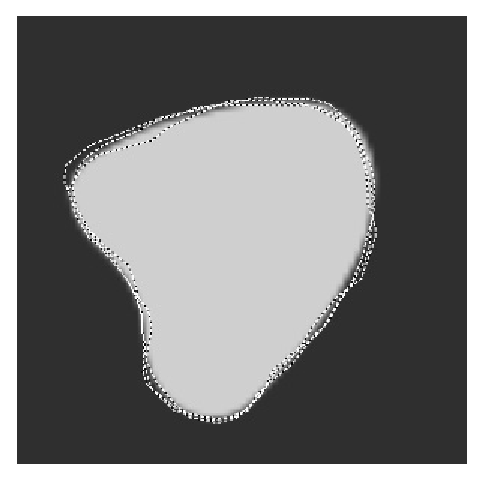
\includegraphics[height=7cm]{mcr3b.eps}
   \end{tabular}
   \end{center}
   \caption[example] 
%>>>> use \label inside caption to get Fig. number with \ref{}
   { \label{fig:example} 
Blah Blah.}
   \end{figure} 
%-------------
%%%%%%%%%%%%%%%%%%%%%%%%%%%%%%%%%%%%%%%%%%%%%%%%%%%%%%%%%%%%%
\acknowledgments     %>>>> equivalent to \section*{ACKNOWLEDGMENTS}       
The authors would like to extend a special thanks to the United States Geological Survey (USGS) for its sponsorship that has made this effort possible.
%%%%%%%%%%%%%%%%%%%%%%%%%%%%%%%%%%%%%%%%%%%%%%%%%%%%%%%%%%%%%
%%%%% References %%%%%

\bibliography{/Users/javier/Desktop/Javier/PHD_RIT/Latex/javier_bib}   
\bibliographystyle{spiebib}   %>>>> makes bibtex use spiebib.bst


\end{document} 
